\section{Implementation}%
\label{sec:implementation}
We have implemented a full-featured prototype of HyperPS.


\subsection{HyperPS Space}%
\label{sub:hyperps_space}
In this paper, HyperPS creates a delicate kernel-level secure and isolated execution space, called HyperPS Space, to inherit privileges of managing physical memory that originally belonged to the compromised hypervisor. 
Figure \ref{fig:address} describes the address layout of HyperPS.  

\begin{figure}[htpb]
    \centering
    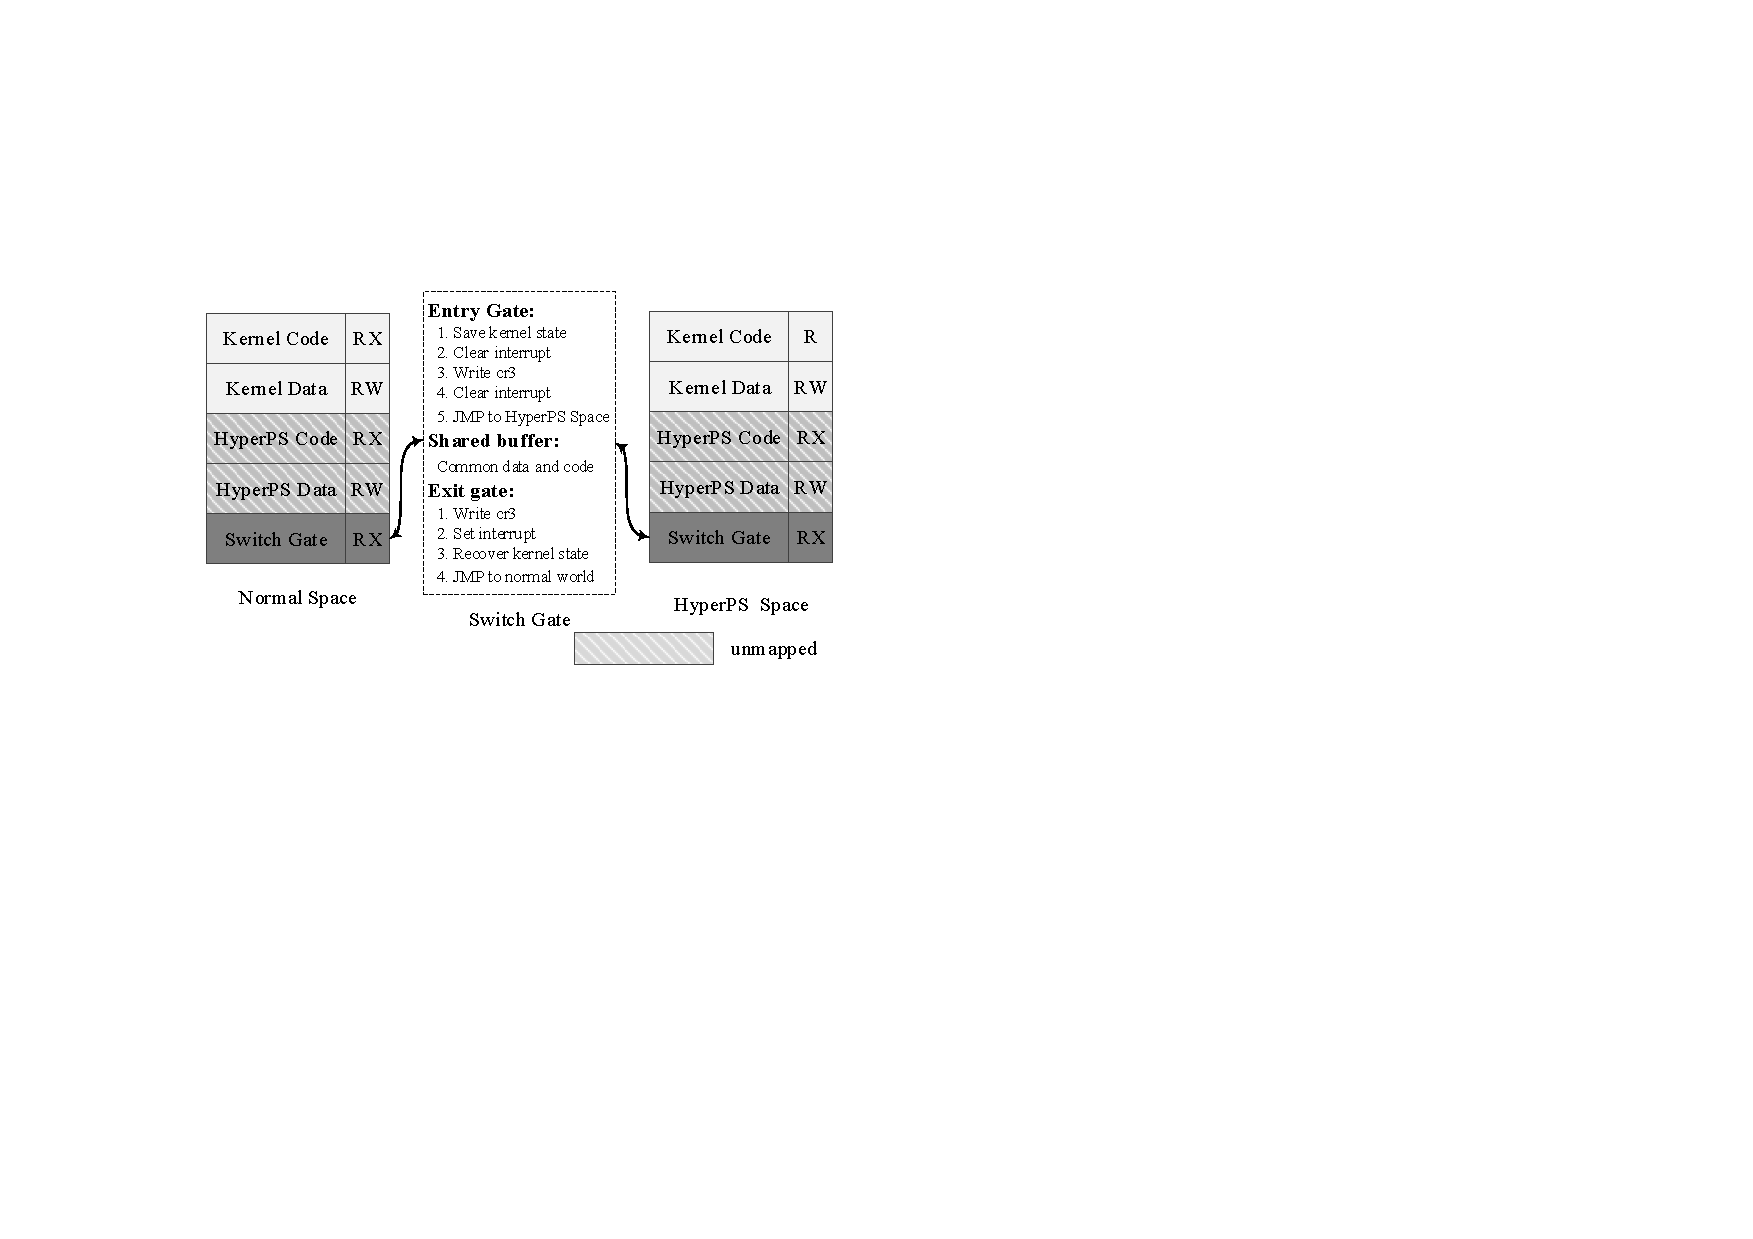
\includegraphics[width=0.8\linewidth]{IMG/address.pdf}
    \caption{Address layout of HyperPS}%
    \label{fig:address}
\end{figure}

As shown in the Figure \ref{fig:address}, HyperPS creates the delicate kernel-level secure and isolated execution space by using two sets of page tables. 
On the left side of Figure \ref{fig:address}, the normal page table contains code and data of the HostOS kernel world. However, page table entries about the HyperPS Space haved been removed from this table. On the other side of Figure \ref{fig:address}, 


except for that of HyperMI World. This can prevent compromised hypervisor from breaking the integrity of HyperMI World. Programs running in normal world can not access data in HyperMI World. On the right of Figure \ref{fig2}, all address is mapped in HyperMI page table.


\iffalse
 We use two isolated address spaces based on two sets of page tables to achieve isolation of HyperMI World.
Figure \ref{fig2} describes the address space layout of two worlds through two sets of page table, the normal page table and HyperMI page table. On the left of Figure \ref{fig2}, the normal page table contains code and data of the normal world except for that of HyperMI World. This can prevent compromised hypervisor from breaking the integrity of HyperMI World. Programs running in normal world can not access data in HyperMI World. On the right of Figure \ref{fig2}, all address is mapped in HyperMI page table.
HyperMI code remains executable and HyperMI data remains writable. What's the most important, kernel code is forbid to execute when HyperMI World is active, so that it can not attack HyperMI World.

\textbf{Creating Switch Gate}
In the middle of Figure \ref{fig2}, the switch gate includes entry/exit gate and shared buffer. Entry gate provides the only entrance to HyperMI World and the exit gate provides the address for returning to the normal world. The shared buffer contains common data and code in normal world and HyperMI World. Common code is switch code, common data is entrance address to HyperMI World and return address to the normal world. The switch gate is mapped at the same place in the normal world and HyperMI World because the switch gate code must be called by the two worlds before and after switching. Of course, the entrance address must be protected after switching to HyperMI World in case that a attacker accesses HyperMI World causally after trusted boot. This is introduced in section \ref{SG}.
\fi


























